\documentclass[a4paper,12pt,twoside,swedish]{report}

%\graphicspath{{figures/}}


\usepackage{times}  
\usepackage{amsmath}
\usepackage{amssymb}
\usepackage{graphicx}
\usepackage{theorem}
\usepackage[latin1]{inputenc}
\usepackage{latexsym}
\usepackage{url}
\usepackage{babel}

\headsep          0.25in
\headheight       12pt
\setlength{\topmargin}{-\headsep}
\addtolength{\topmargin}{-\headheight}
\oddsidemargin      0in
\evensidemargin     0in
\setlength{\textwidth}{\paperwidth}
\addtolength{\textwidth}{-2.0in}
\setlength{\textheight}{\paperheight}
\addtolength{\textheight}{-2.0in}
\addtolength{\textheight}{-1\topskip}
\divide\textheight  by \baselineskip
\multiply\textheight  by \baselineskip
\addtolength{\textheight}{\topskip}

\addto\captionsswedish{
  \renewcommand{\contentsname}
    {Inneh�llsf�rteckning}
}

\begin{document}

\pagestyle{empty}

%----------------------------- Front matter of the document

\title{Amazeballs}

\date{2014-03-03}
\author{Sofie Lindblom, Anton Arbring, David Lindh}

\maketitle

\begin{abstract}
I kursen TNM085, modelleringsprojekt skapas ett projekt vars syfte �r att modellera ett fysikaliskt system av valfri typ. I den h�r rapporten kan du l�sa om hur x antal kolliderande studsbollar simuleras. Inspirationen �r h�mtad fr�n en reklam Sony gjorde 2009 d�r man sl�pper miljontals studsbollar ner f�r en gata i San Francisco.  
\vfill
\end{abstract}

\tableofcontents  % chapter with the table of contents
\addtocontents{toc}{\protect\thispagestyle{empty}}
\listoffigures    % chapter with the list of figures
\addtocontents{lof}{\protect\thispagestyle{empty}}

%----------------------------- Body of the document

\pagestyle{plain}

\chapter{Inledning}
\setcounter{page}{1}

\section{Inledning}
Efter att ha resonerat kring att simulera luftballonger, rinnande vatten eller r�k landade gruppen tillslut i beslutet att simulera studsbollar. Motiveringen till beslutet var att det p� ett smidigt s�tt skulle g� att involvera interaktivitet genom att anv�ndaren kan v�lja utvalda attribut som till exempel radien p� studsbollen. Huvudsakligt fokus har varit en fysikaliskt realistisk studs mellan bollar och omgivning samt kollisionshanteringen mellan bollarna. Sekund�rt fokus har varit interaktivitet och en mer komplex omgivning.
\begin{itemize}
\item In Catilinam I
\item In Catilinam II
\item In Catilinam III
\item In Catilinam IV
\end{itemize}
Est mihi iucunda in


\section{Syfte}

Syftet med projektet �r att implementera utvalda fysikaliska samband i en realistisk teknisk simulering. Vidare har projektrapporten skrivits i verktyget LaTex och d�rmed har �ven dessa kunskaper utvecklats.  Ett �vergripande syfte har varit f�r studenterna att v�ga olika tillv�gag�ngss�tt och metoder mot varandra f�r att v�lja det som �r b�st l�mpat f�r projektets resultat.

\chapter{Implementation}

 


\begin{table}[htbp]
  \caption{Heading centred.}
  \label{table_example}
  \begin{tabular*}{\hsize}{lllll}
\hline
Xxxxx & Xxxxx & Xxxx & Xxxxx & Xxxxx \\
      &       &      &       & xxxx  \\
\hline
X     & X     &      & XXX   &       \\
XX    & XXX   & XX   & X     & XX    \\
XXX   & X     & X    & XXX   & XXX   \\
XXXX  & XX    &      & XX    & X     \\
X XX  & XXX   & XX   & XXX   & XXXXX \\
\hline
  \end{tabular*}
\end{table}


\begin{figure}
\begin{center}
    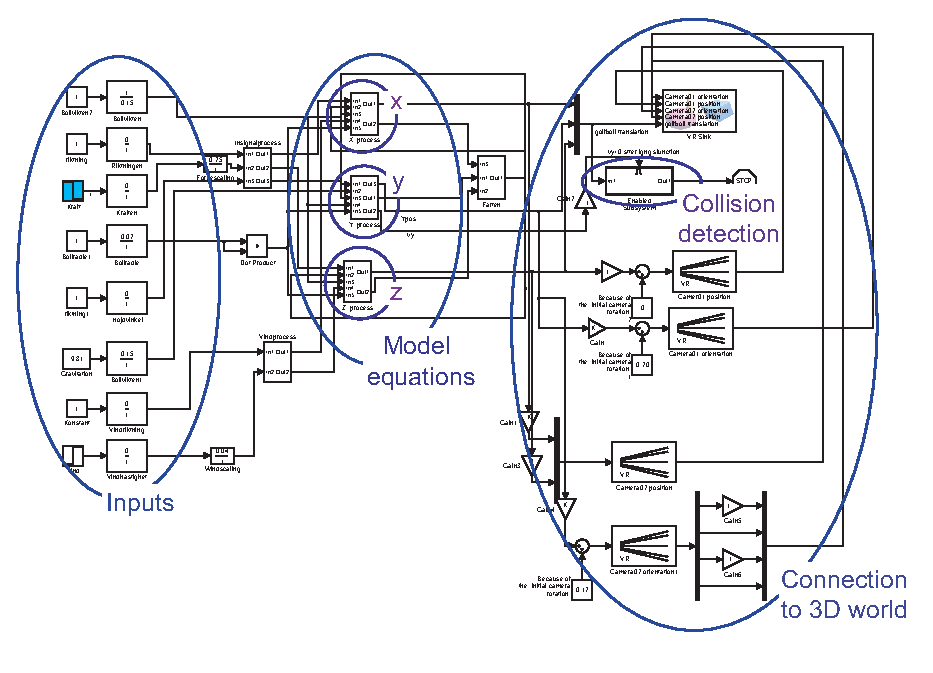
\includegraphics[width=11cm]{Figures/block_simulink.eps} 
\end{center}
\caption{Example of figure}
\label{model_block}
\end{figure}

Figure \ref{model_block} is not by Cicero.
Multa meo quodam dolore in vestro timore sanavi. Nunc si hunc exitum


\section{F�rarbete}
Some words might be appropriate describing equation \ref{e1}, if we
had but time and space enough.
\begin{equation}
\frac{\partial F}{\partial
t}=D\frac{\partial^2 F}{\partial x^2},
\label{e1}
\end{equation}
Quare, patres conscripti, consulite vobis, prospicite patriae,


\section{Simuleringar i MATLAB}
Also containing some text, and a figure (\ref{fig:plot_result}).
\begin{figure}
 \begin{center}
   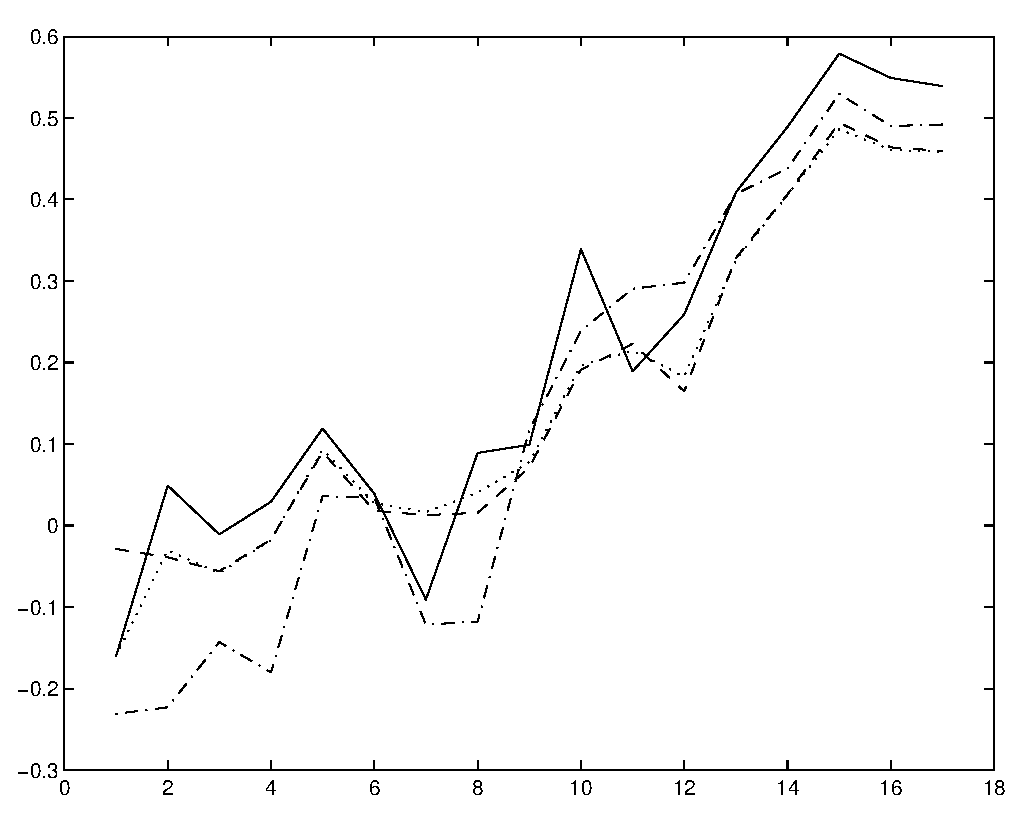
\includegraphics[width=7cm]{Figures/result.eps}  
  \end{center}
\caption{Another figure example}
   \label{fig:plot_result}
\end{figure}

\subsection{1D}
Bla Bla

\subsection{2D}
Bla Bla

\subsection{3D}
Bla Bla


\section{Simuleringar i WebGL}
A word or two to conclude,  and this even includes some
inline maths: \(R(x,t)\sim
t^{-\beta}g(x/t^\alpha)\exp(-|x|/t^\alpha)\)


\chapter{Implementation}
\section{F�renklingar}
\section{Resultat}
\section{Reflektion}

 Ego multa tacui, multa pertuli, multa concessi,



%----------------------------- Back matter of the document

\bibliographystyle{vancouver}
\bibliography{bibsam}

\addcontentsline{toc}{chapter}{Litteraturf�rteckning}

\pagestyle{empty}

\appendix

\chapter{Proof of\dots}

\label{app:proof1}

\thispagestyle{empty}

Proof\dots

Bla 1

\chapter{Second proof of\dots}

\label{app:proof2}

\thispagestyle{empty}

bla2

\end{document}

